%%%
%%% 编译此TeX文件需要完整的ctex宏集(建议使用TeXLive/MikTeX最新版本配置所需宏)以及所有\usepackage[*]{...}
%%% 命令中需要的名称为...的包
%%% 使用XeLaTeX引擎编译
%%%
\documentclass[8pt]{ctexbeamer}

%	Beamer主题
\usetheme{boxes}
%	Beamer颜色主题
\usecolortheme{seahorse}
%	Beamer内置主题
\useinnertheme{rectangles}
%	Beamer外置主题
\useoutertheme[subsection=false,footline=authortitle]{miniframes}
%	Beamer字体主题
\usefonttheme{default}
\usefonttheme[onlymath]{serif}						%	数学字体主题
%	Beamer导航栏
\setbeamertemplate{navigation symbols}[horizontal]	%	设置导航栏为水平
%	Beamer目录
\setbeamertemplate{section in toc}[square]			%	目录章节设置为方块
%	Beamer无序列表模板
\definecolor{SteelBlue}{RGB}{70,130,180}
\setbeamertemplate{itemize item}[square]			%	使用三角符号进行无序列表枚举
\setbeamercolor{itemize item}{fg=SteelBlue}			%	无序列表itemize环境颜色	
%	Beamer标准块环境
\setbeamercolor{block title}{bg=cyan!50, fg=black}		%	标题颜色
\setbeamercolor{block body}{bg=cyan!10}				%	块主体颜色
%	Beamer章节页设置
\AtBeginSection{
	\begin{frame}
		\begin{beamercolorbox}[sep=25pt,center]{part title}
			{\LARGE	\insertsection}
		\end{beamercolorbox}
	\end{frame}
}

%	集成所需宏
\usepackage{enumerate}							%	枚举环境
\usepackage{graphicx}							%	图片插入
\usepackage{amsmath,amsthm,amsfonts,amssymb}    %	使用AMS集成包
\usepackage{xcolor}     						%	颜色
\usepackage{hyperref}							%	超链接

%  文本提示框
\usepackage{tcolorbox}
\tcbuselibrary{skins}
\tcbsetforeverylayer{enhanced}
\newtcolorbox[auto counter,number within=section]{notebox}[1]{
    skin=empty,
    top = 0pt,
    bottom = 0pt,
    toprule = 0pt,
    bottomrule = 0pt,
    leftrule = 0pt,
    rightrule = 0pt,
    borderline west={2pt}{0pt}{#1},
}

% 注释结论
\newenvironment{remark}
{
	\begin{notebox}{orange}
}
{
	\end{notebox}
}

% 引用结论
\renewenvironment{quote}
{
	\begin{notebox}{gray}
}
{
	\end{notebox}
}


\title{华为第一届领航杯应用数学大赛}
\subtitle{低功耗自适应FIR滤波硬件算法}
\date{2023.9.20}
\author{柴昊、李明昊、王熙元}
\institute{复旦大学\\
	南京大学}

%\logo[options]{logo path}	添加LOGO

\begin{document}

% Title page 
\begin{frame}[plain, noframenumbering]
	\titlepage
\end{frame}

\begin{frame}[plain]
	\begin{beamercolorbox}[sep=12pt,center]{part title}
		{\Large	\contentsname}		
	\end{beamercolorbox}
    \tableofcontents
\end{frame}

\section{理论回顾}


\begin{frame}{算法复现}
	\begin{quote}
		文章来源:
		
		reference1

		reference2

		reference3

	\end{quote}
	主要内容:

	使用经典加速

	\begin{itemize}
		\item AAA
		\item BBB
		\item CCC
	\end{itemize}

	DDDDDDD

\end{frame}


\section{算法实现}

\begin{frame}{C++硬件算法}
	ADDDDAADDADADADADADAD

	\begin{block}{AAA}
		测试方式
	\end{block}
	\begin{quote}
		文件树
		evaluation.h
		evaluation.cpp
		.....

	\end{quote}
\end{frame}

\begin{frame}{大标题}{子标题}
	\begin{columns}
		% Column 1
		\begin{column}{0.5\textwidth}
			\begin{figure}
				\centering
					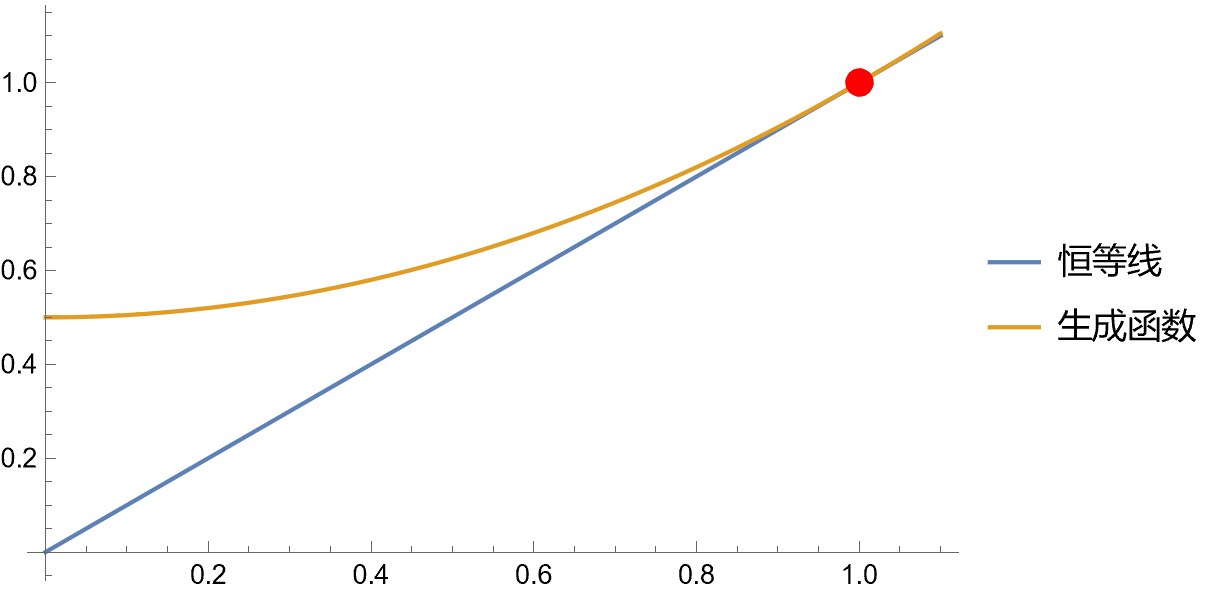
\includegraphics[width=0.9\textwidth]{figure/P1.png}
					\caption{图一}
			\end{figure}
		\end{column}
		% Column 2    
		\begin{column}{0.5\textwidth}
			\begin{figure}
			\centering
				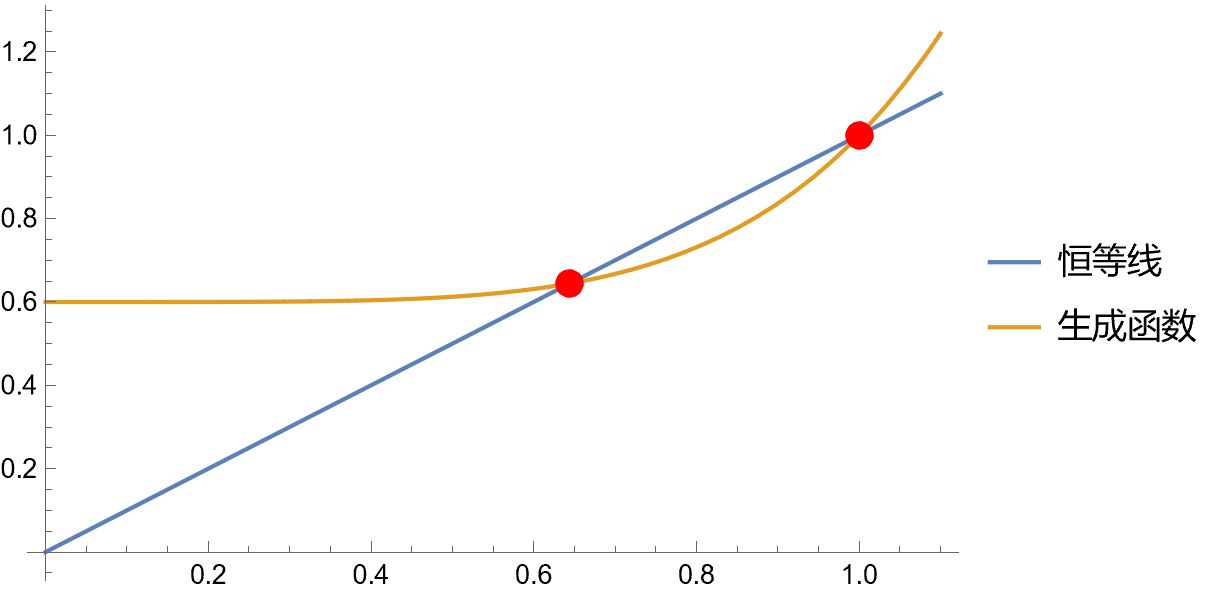
\includegraphics[width=0.9\textwidth]{figure/P2.png}
				\caption{图二}
			\end{figure}
		\end{column}
		\end{columns}
\end{frame}


\section{硬件测试}


\begin{frame}{数据表格}
	AAAAAA 数学公式 BBBBBBB
	\begin{equation*}
		G_1 (x) = p_0 + \cdots + p_5 x^5, \quad G_2(x) = f + (1-f)e^{-N_2 (1-x)}
	\end{equation*}
	从而
	\begin{align*}
		&\textstyle	\widetilde{Z}(x) = Q + (1-Q) \frac{G_{1}^{'}(T_1 x + (1-T_1))G_2(T_2 x + (1-T_2)) + N_2 G_{1}(T_1 x + (1-T_1))e^{-N_2 T_2(1-x)}}{G_1^{'}(1) + N_2}\\
		&\textstyle	R_0 = Q + (1-Q)\frac{T_1 G_{1}^{''}(1) + (1-f)N_1 N_2 (T_1 + T_2) + (1-f)N_2^2 T_2}{G_1^{'}(1) + N_2}
	\end{align*}
	如下等表格。。。。
	\begin{center}
		\begin{tabular}{|c|c|c|c|}
			国家	&	$R_0$	&	$\mathbf{P}_{\infty}$	& $Z(\mathbf{P}_{\infty})$	\\
			德国	&	2.81	&	0.0852					& 	0.0855					\\
			西班牙	&	3.44	&	0.039					&	0.039					\\
			葡萄牙	&	3.4		&	0.04					&	0.04					\\ 
			巴西	&	3.82	&	0.026					&	0.026					\\
		\end{tabular}
	\end{center}
\end{frame}

\begin{frame}{讨论}
	\begin{remark}
		主要技术优势。。。
	\end{remark}
	\pause
	\begin{remark}
		算法在硬件/通信芯片上的性能提示效率
	\end{remark}

\end{frame}

\section{致谢}

\begin{frame}
	\begin{center}
		\Huge\heiti{报告结束\, 感谢聆听}
	\end{center}
\end{frame}

\end{document}


% %	命令简化
% \newcommand{\Z}{\mathbb{Z}}
% \newcommand{\E}{\mathbb{E}}
% \newcommand{\Prob}{\mathbb{P}}
% \newcommand{\Var}{\mathbf{Var}}
% \newcommand{\R}{\mathbb{R}}
% % 	数学符号Stirling数
% \newcommand{\genstirlingI}[3]{%
%   \genfrac{[}{]}{0pt}{#1}{#2}{#3}%
% }
% \newcommand{\genstirlingII}[3]{%
%   \genfrac{\{}{\}}{0pt}{#1}{#2}{#3}%
% }													%	第一类第二类Stirling数
% \newcommand{\stirlingI}[2]{\genstirlingI{}{#1}{#2}}
% \newcommand{\dstirlingI}[2]{\genstirlingI{0}{#1}{#2}}
% \newcommand{\tstirlingI}[2]{\genstirlingI{1}{#1}{#2}}
% \newcommand{\stirlingII}[2]{\genstirlingII{}{#1}{#2}}
% \newcommand{\dstirlingII}[2]{\genstirlingII{0}{#1}{#2}}
% \newcommand{\tstirlingII}[2]{\genstirlingII{1}{#1}{#2}}
%	Beamer章节页
% \definecolor{C1}{RGB}{0,62,128}
% \definecolor{C2}{RGB}{0,159,227}
% \definecolor{GRAY1}{RGB}{245,245,245}
% \setbeamercolor{titlepage}{fg=GRAY1,bg=C1}		%	颜色使用
% \setbeamertemplate{section page}
% {
% 	\nointerlineskip
% 	\begin{beamercolorbox}[dp=2.3ex, sep=2ex, wd=\paperwidth, ht=\paperheight]{titlepage}
% 		\vbox to 35ex{
% 			\hspace{0.16\linewidth}
% 			\begin{minipage}[c]{0.6\linewidth}
% 				{\Large \bfseries \insertsection}

% 				\begin{tikzpicture}
% 					\draw[line width=0.5pt, color=C2] (0,0) -- (\linewidth,0);
% 				\end{tikzpicture}
% 			\end{minipage}
% 		}
% 	\end{beamercolorbox}
% }
%

%	补充所需宏
%\usepackage{mdframed}       					%	用mdframe设置定理样式
%\usepackage{zref}								%	引用格式翻新
%\usepackage{tikz-cd}							%	tikz绘图
%\usepackage{verbatim}							%	代码输入等